\documentclass[a4paper,11pt]{report}
\usepackage[utf8x]{inputenc}
\usepackage{amsmath} % AMS Math Package
\usepackage{amsthm} % Theorem Formatting
\usepackage{amssymb}	% Math symbols such as \mathbb
\usepackage[pdftex]{graphicx} % Allows for eps images
%\usepackage{multicol} % Allows for multiple columns
%\usepackage[dvips,letterpaper,margin=2in,bottom=2in]{geometry}
%\usepackage{geometry}
\usepackage{booktabs}
\usepackage{enumerate}
\usepackage{verbatim}
\usepackage{fancyhdr}
\usepackage{titlesec}
\usepackage{longtable}
\usepackage{subfigure}
\usepackage{hyperref}
\usepackage{float}
\pagestyle{fancy}
\usepackage[italian]{babel}
\usepackage{graphicx}
\usepackage{latexsym}
\usepackage{verbatim} % commenti estesi
\usepackage{geometry}
\geometry{a4paper,top=3cm,bottom=3cm,left=2.5cm,right=2.5cm,%
heightrounded,bindingoffset=5mm}
\fancyhf{}
%\fancyhead[LE,RO]{\slshape \rightmark}
\fancyhead[LO,RE]{\slshape \leftmark}
\fancyfoot[C]{\thepage}
%\titleformat{\chapter}%
%[display]{\vspace{2cm}\Large\bfseries}{\Huge\thechapter \ \hrulefill}{0pt}{\vspace{4mm}}%
%{\Large\bfseries\filcenter}

%%%%%%%%%%%%%%%%%%%%%%%%%%%%%%%%%%%%%%%%%%%%%%%%%%%%%%%%%%%%%%%%%%%%%%%%%%%%%%%%%%%%%%%%%%%%%%%%%%%%%%%%%%%%%%%%%%%%%%%%%%%%%%%%%%%%%%%%
%Mathematical Commands
%%%%%%%%%%%%%%%%%%%%%%%%%%%%%%%%%%%%%%%%%%%%%%%%%%%%%%%%%%%%%%%%%%%%%%%%%%%%%%%%%%%%%%%%%%%%%%%%%%%%%%%%%%%%%%%%%%%%%%%%%%%%%%%%%%%%%%%%%%
 % Sets margins and page size
%\pagestyle{empty} % Removes page numbers
\makeatletter % Need for anything that contains an @ command
% \DeclareMathOperator{\Sample}{Sample}
\let\vaccent=\v % rename builtin command \v{} to \vaccent{}
\renewcommand{\v}[1]{\ensuremath{\mathbf{#1}}} % for vectors
\newcommand{\gv}[1]{\ensuremath{\mbox{\boldmath$ #1 $}}}
% for vectors of Greek letters
\newcommand{\uv}[1]{\ensuremath{\mathbf{\hat{#1}}}} % for unit vector
\newcommand{\abs}[1]{\left| #1 \right|} % for absolute value
\newcommand{\avg}[1]{\left< #1 \right>} % for average
\let\underdot=\d % rename builtin command \d{} to \underdot{}
\renewcommand{\d}[2]{\frac{d #1}{d #2}} % for derivatives
\newcommand{\dd}[2]{\frac{d^2 #1}{d #2^2}} % for double derivatives
\newcommand{\pd}[2]{\frac{\partial #1}{\partial #2}}
% for partial derivatives
\newcommand{\pdd}[2]{\frac{\partial^2 #1}{\partial #2^2}}
% for double partial derivatives
\newcommand{\pdc}[3]{\left( \frac{\partial #1}{\partial #2}
 \right)_{#3}} % for thermodynamic partial derivatives
\newcommand{\ket}[1]{\left| #1 \right>} % for Dirac bras
\newcommand{\bra}[1]{\left< #1 \right|} % for Dirac kets
\newcommand{\braket}[2]{\left< #1 \vphantom{#2} \right|
 \left. #2 \vphantom{#1} \right>} % for Dirac brackets
\newcommand{\matrixel}[3]{\left< #1 \vphantom{#2#3} \right|
 #2 \left| #3 \vphantom{#1#2} \right>} % for Dirac matrix elements
\newcommand{\grad}[1]{\gv{\nabla} #1} % for gradient
\let\divsymb=\div % rename builtin command \div to \divsymb
\renewcommand{\div}[1]{\gv{\nabla} \cdot #1} % for divergence
\newcommand{\curl}[1]{\gv{\nabla} \times #1} % for curl
\let\baraccent=\= % rename builtin command \= to \baraccent
\renewcommand{\=}[1]{\stackrel{#1}{=}} % for putting numbers above =
\newtheorem{prop}{Proposition}
\newtheorem{thm}{Theorem}[section]
\newtheorem{lem}[thm]{Lemma}
\theoremstyle{definition}
\newtheorem{dfn}{Definition}
\theoremstyle{remark}
\newtheorem*{rmk}{Remark}
\newcommand{\p}[2]{ \frac{ \partial #1}{ \partial #2}} %derivata partiale
\newcommand{\lap}{\nabla^2} %laplaciano
\newcommand{\ham}{\mathcal{H}} % Simbolo dell'hamiltoniana
\newcommand{\rint}{\int_\mathbb{R}} % Integrale su R
\newcommand{\modq}[1]{| #1|^2} % Modulo quadro di ``argomento''
\newcommand{\navg}[2]{\left< #1 ^{#2} \right>} %media di ``arg''^n
\newcommand{\con}[1]{\overline{#1}} %coniugato con la barra
\newcommand{\ih}{\frac{i}{\hbar}} % i/h tagliato
\newenvironment{sistem}%
{\left\lbrace\begin{array}{@{}l@{}}}%
{\end{array}\right.}

\newenvironment{myfig}[1][]{%
\begin{center}%
 \begin{figure}[#1]%
  \centering%
  }{%
  \end{figure}%
  \end{center}%
  }




\begin{document}

\newcommand{\HRule}{\rule{\linewidth}{0.5mm}}
\begin{titlepage}
 \begin{center}
  \HRule \\[0.4cm]
{ \huge \bfseries Laboratorio di \\
fisica computazionale}\\[0.4cm]
\HRule \\[1cm]
\begin{flushleft} \Large
Carlo \textsc{Sana} 
\end{flushleft}

\begin{flushright} \Large
	mat. 726409
\end{flushright}
\HRule \\[1cm]
%\begin{flushright}
%\includegraphics[width=0.7\textwidth,]{title.png}
%\end{flushright}

\end{center}

\end{titlepage}

\tableofcontents 
\newpage
\section{Modello di Ising}
Il modello è stato implementato su un reticolo bidimensione di larghezza N e inizializzando gli spin al valore $\pm 1 $  con uguale probabilità.
Sono stati implementati due algoritmi: Metropolis e Swendsen-Wang.\\

\subsection{Termalizzazione}
Possiamo valutare quando avviene la corretta termalizzazione del sistema analizzando l'andamento della magnetizzazione e dell'energia in funzione del tempo markoviano.
Di seguito è riportato l'andamento dell'energia e della magnetizzazione durante la termalizzazione a due diverse temperature.
\subsubsection*{Metropolis}
\begin{figure}[h]
\subfigure[$\beta=0.3$]{
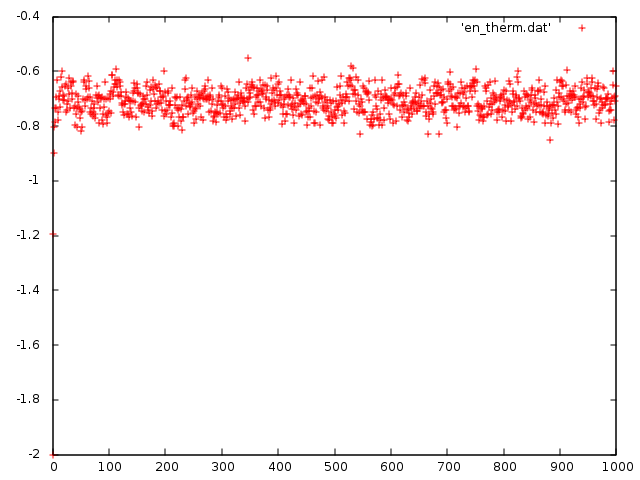
\includegraphics[scale=0.45]{metropolis/en_therm.png}
}
\subfigure[$\beta=0.453$]{
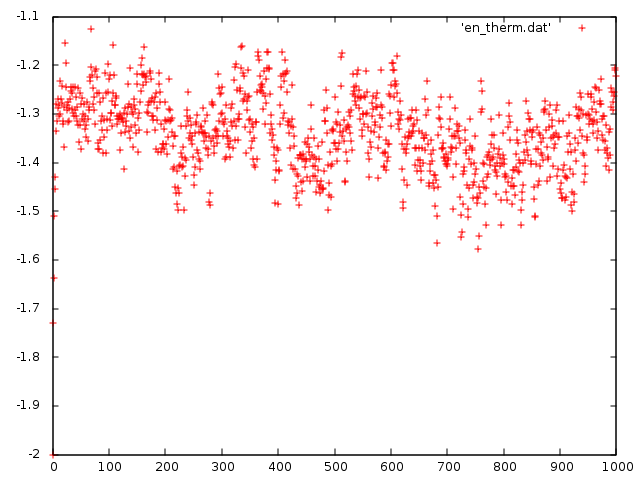
\includegraphics[scale=0.45]{metropolis/en_therm_crit.png}
}
\caption{Energia (Metropolis)}
\end{figure}
\begin{figure}[h]
\subfigure[$\beta=0.3$]{

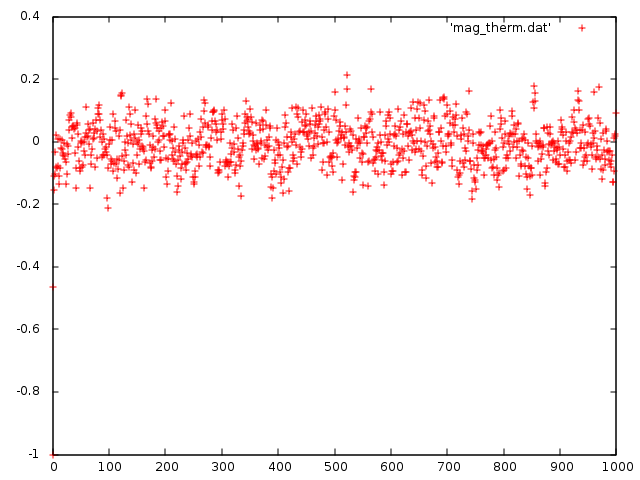
\includegraphics[scale=0.45]{metropolis/mag_therm.png}
}
\subfigure[$\beta=0.453$]{

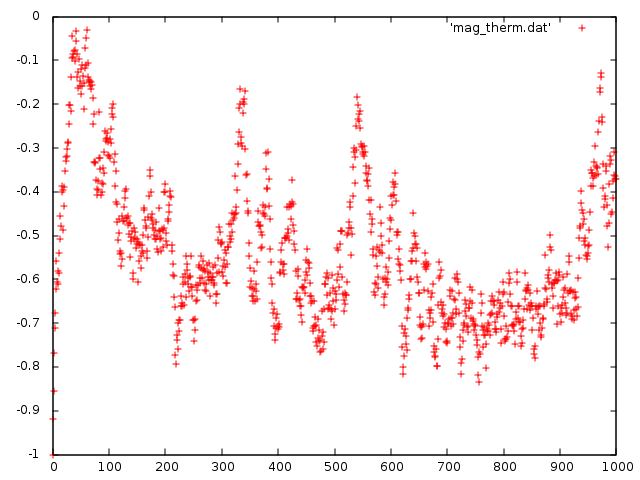
\includegraphics[scale=0.45]{metropolis/mag_therm_crit.png}
}
\caption{Magnetizzazione  (Metropolis)}
\end{figure}
Come si può vedere dal grafico relativo alla magnetizzazione a $\beta=0.453$, vicino al punto critico il tempo di termalizzazione cresce di molto. Esso rimane comunque intorno a 100 alla temperatura critica.
Dopo l'analisi di questi dati si è deciso di fissare il tempo di termalizzazione a 1000 passi temporali.
\subsubsection*{Swendsen-Wang}
\begin{figure}[h]
\subfigure[$\beta=0.3$]{
	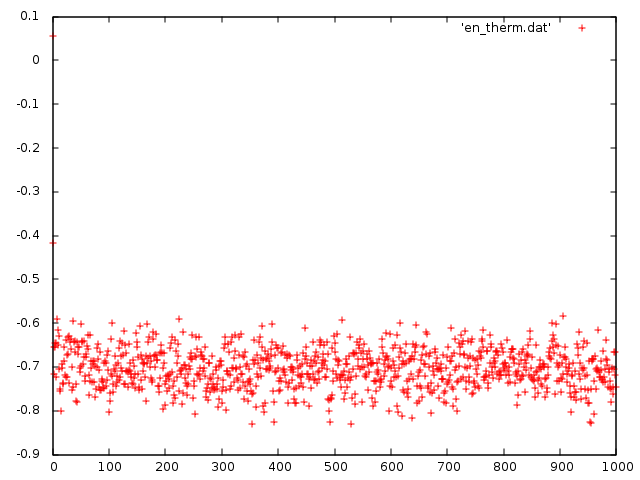
\includegraphics[scale=0.45]{sw/en_therm0-3.png}
}
\subfigure[$\beta=0.453$]{
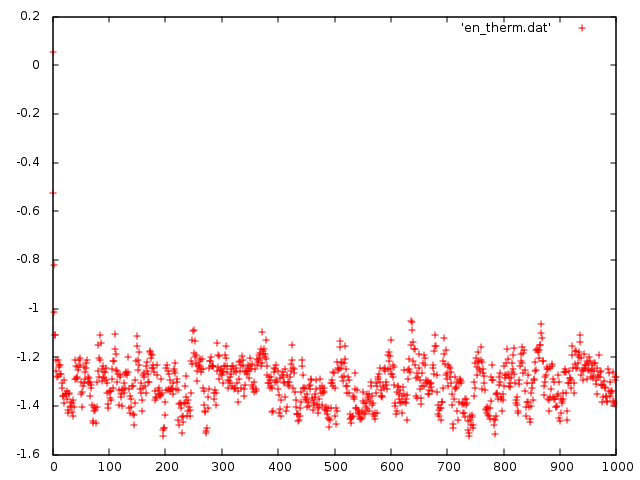
\includegraphics[scale=0.45]{sw/en_therm0-43.png}
}
\caption{Energia (Swendsen-Wang) }
\end{figure}

\begin{figure}[h]
\subfigure[$\beta=0.3$]{
	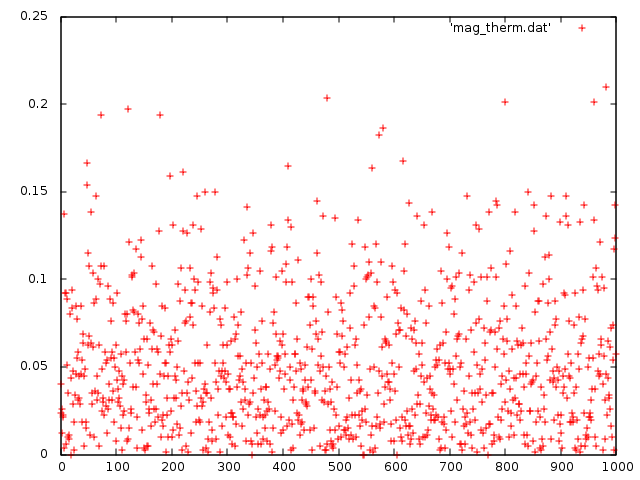
\includegraphics[scale=0.45]{sw/mag_therm0-3.png}
	}
\subfigure[$\beta=0.453$]{
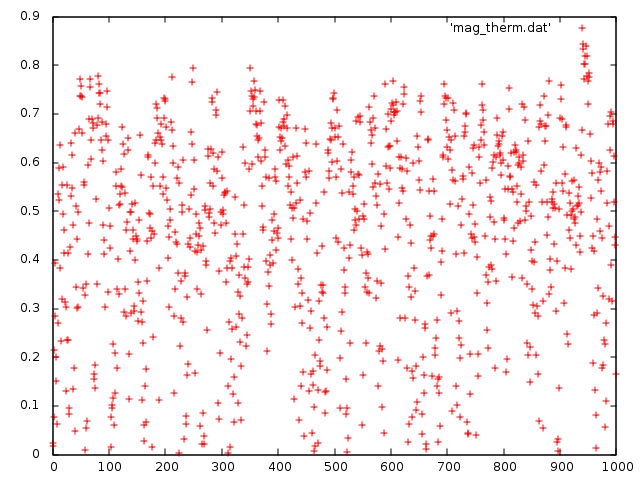
\includegraphics[scale=0.45]{sw/mag_therm0-43.png}
}
\caption{Magnetizzazione  (Swendsen-Wang)}
\end{figure}
Anche con questo algoritmo, il tempo di termalizzazione è molto minore dei 1000 passi utilizzati per far termalizzare il sistema nel programma.
La sostanziale differenza che si vede nei grafici relativi alla magnetizzazione vicino al punto critico è dovuta all'inefficienza dell'algoritmo Metropolis nell'estrarre configurazioni scorrelate vicino al punto critico, fenomeno solitamente chiamato \emph{critical slowing down}.
Esso si manifesterà più chiaramente nello studio dell'autocorrelazione delle configurazioni.


\subsection{Autocorrelazione fra le configurazioni}
Come in ogni simulazione Monte Carlo, è necessario studiare l'autocorrelazione delle configurazione estratte attraverso l'algoritmo in modo da stimare l'efficienza dell'algoritmo ad estrarre configurazioni
indipendenti e quindi nel produrre statistica.\\
Il tempo di autocorrelazione è stato calcolato utilizzando la formula:
$$
	\tau_{corr} = \frac{1}{2} + \sum_{t=1}^{t_{max}} \Gamma(t) \qquad \mbox{dove} \; \Gamma \; \mbox{è la funzione di autocorrelazione}
$$
Gli errori sono stati stimati ripetendo le misure (in questo grafico 12 volte).
Non è stato possibile stimare il valore di $\tau_{corr}$ attraverso un fit con una funzione del tipo $e^{-\frac{t}{\tau_{c}}}$ in quanto vicino al punto critico l'autocorrezione smette di avere questo andamento esponenziale che ha lontano dal punto critico.
\begin{figure}[h]
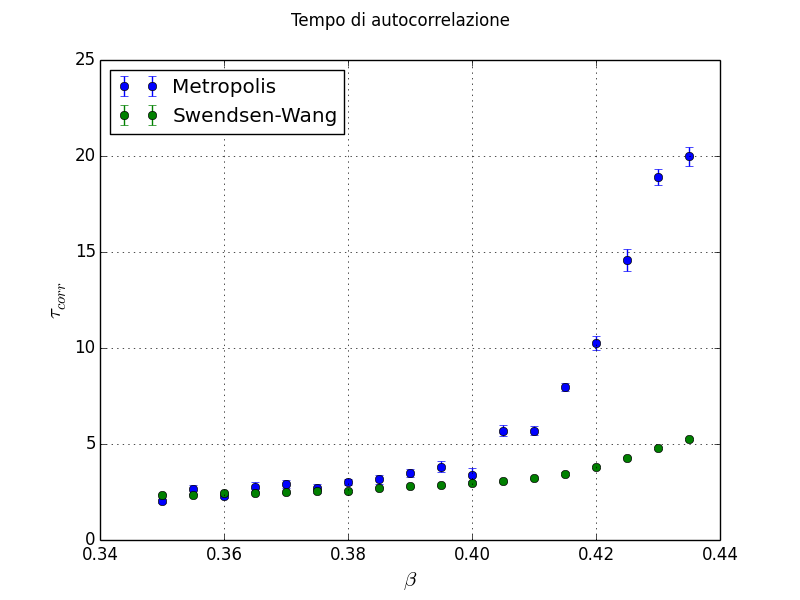
\includegraphics[scale=0.6]{compare.png}
\caption{Tempo di autocorrelazione dell'energia con N=46.}
\end{figure}
Come si può vedere dai grafici, l'algoritmo Metropolis ha un tempo di autocorrelazione nettamente più elevato rispetto a Swendsen-Wang. Questo diverso comportamento è dovuto principalmente al fatto che Metropolis è un algoritmo locale, ossia l'inversione di ogni spin dipende esclusivamente dagli spin circostanti ad esso. L'algoritmo di Swendsen-Wang invece, è non-locale a causa della taglia estesa  che i cluster possono assumere.
Questo permette a questo algoritmo di non avere difficoltà ad estrarre configurazioni statisticamente scorrelate più velocemente rispetto a Metropolis.

\subsection{Binning}
Prima di affrontare la misura di osservabili è necessario analizzare come affrontare la correlazione fra le configurazioni estratte dagli algoritmi.
La tecnica migliore per ovviare a questo fatto è quella del \emph{binning}, ossia raggruppare misure in intervalli di larghezza abbastanza grande da diventare un gruppo di misure scorrelate tra loro.
A questo punto si procede a fare la media in ogni intervallo e si hanno così $\frac{N}{m}$ misure statisticamente indipendenti fra loro, a partire da $N$ misure autocorrelate suddivise in intervalli di larghezza $m$.\\
\'E fondamentale scegliere la larghezza corretta dell'intervallo. Ciò può essere fatto valutando l'andamento
della deviazione standard della media del nuovo set di $\frac{N}{m}$ misure in funzione di $m$.
Come si può immaginare, la larghezza del bin è associata al tempo di autocorellazione di cui si è parlato prima. 

\subsubsection*{Metropolis}
Si vedano ora alcuni grafici di questa quantità a diverse temperature e per due diverse osservabili.
\begin{figure}[h!]
\subfigure[Energia a $\beta=0.325$]{
	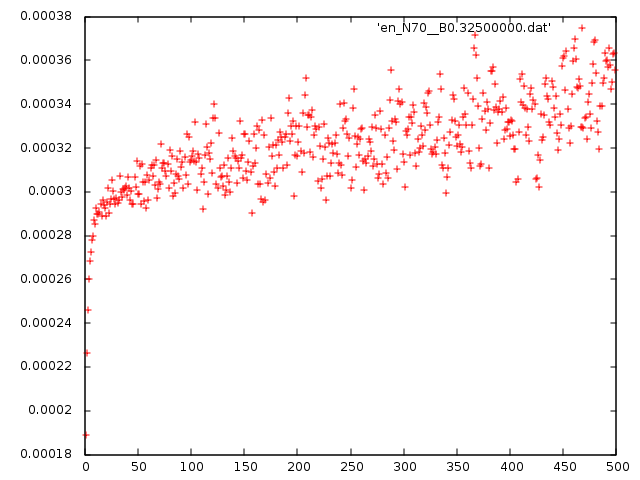
\includegraphics[scale=0.45]{metropolis/bin_en_0325.png}
}
\subfigure[Energia $\beta=0.4508$]{
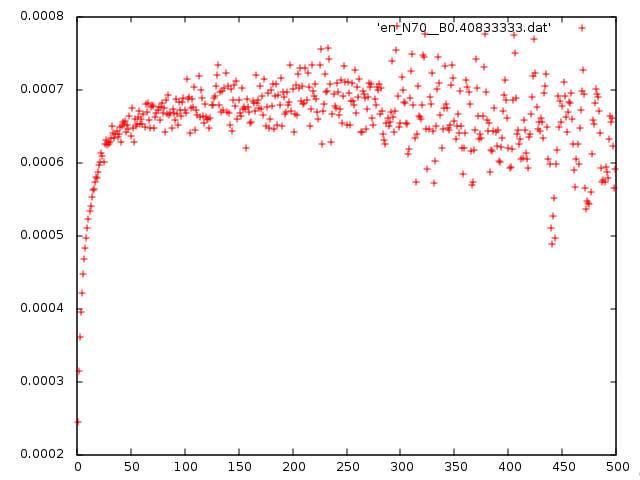
\includegraphics[scale=0.45]{metropolis/bin_en_0408.png}
}
\caption{Deviazione standard dell'energia in funzione della larghezza dei \emph{bin} }
\end{figure}
\begin{figure}[h!]
\subfigure[Energia a $\beta=0.453$]{
	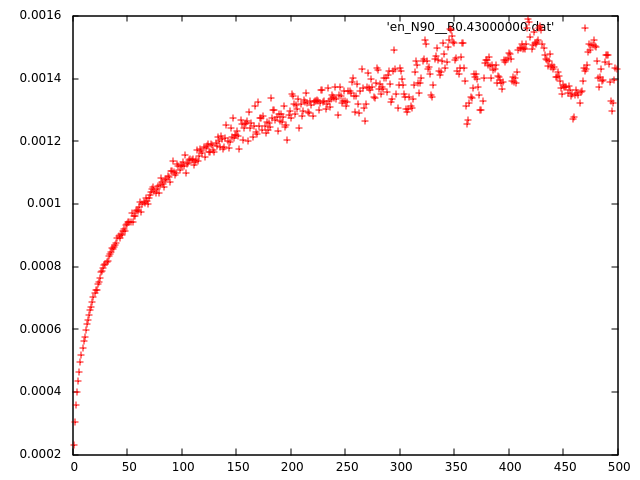
\includegraphics[scale=0.45]{metropolis/bin_en_043.png}
}
\subfigure[Energia $\beta=0.459$]{
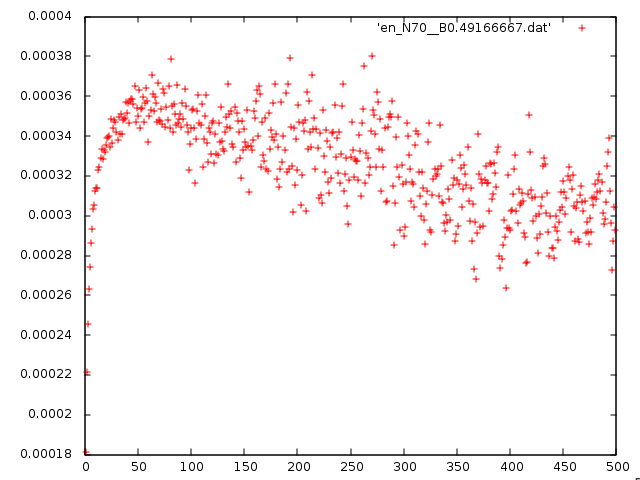
\includegraphics[scale=0.45]{metropolis/bin_en_049.png}
}
\caption{Deviazione standard dell'energia in funzione della larghezza dei \emph{bin} }
\end{figure}

\begin{figure}[h!]
\subfigure[Magnetizzazione a $\beta=0.325$]{
	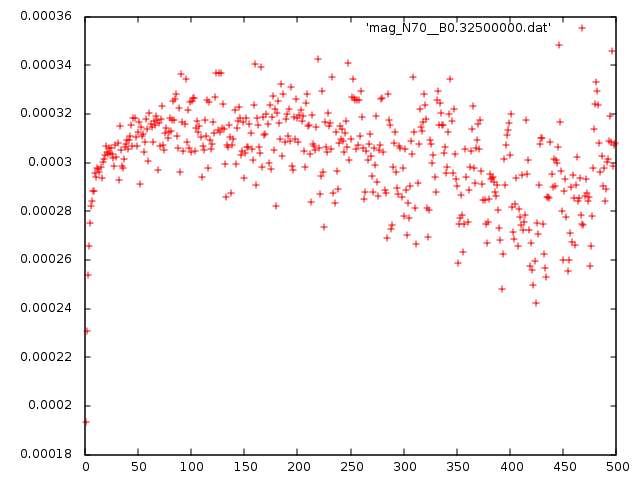
\includegraphics[scale=0.45]{metropolis/bin_mag_0325.png}
}
\subfigure[Magnetizzazione $\beta=0.4508$]{
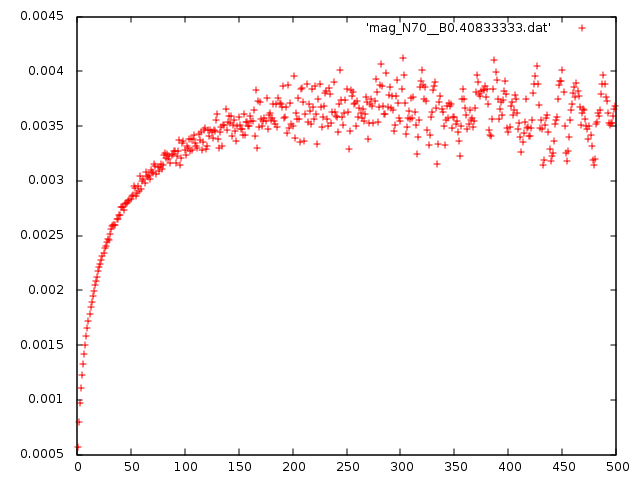
\includegraphics[scale=0.45]{metropolis/bin_mag_0408.png}
}
\caption{Deviazione standard della magnetizzazione in funzione della larghezza dei \emph{bin} }
\end{figure}
\begin{figure}[h!]
\subfigure[Magnetizzazione a $\beta=0.43$]{
	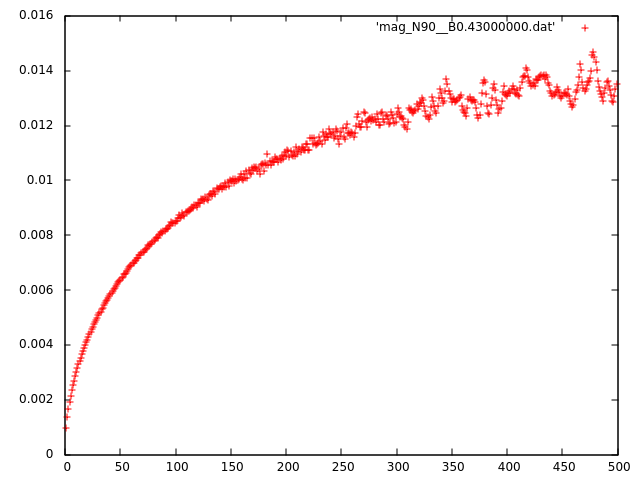
\includegraphics[scale=0.45]{metropolis/bin_mag_043.png}
}
\subfigure[Magnetizzazione $\beta=0.49$]{
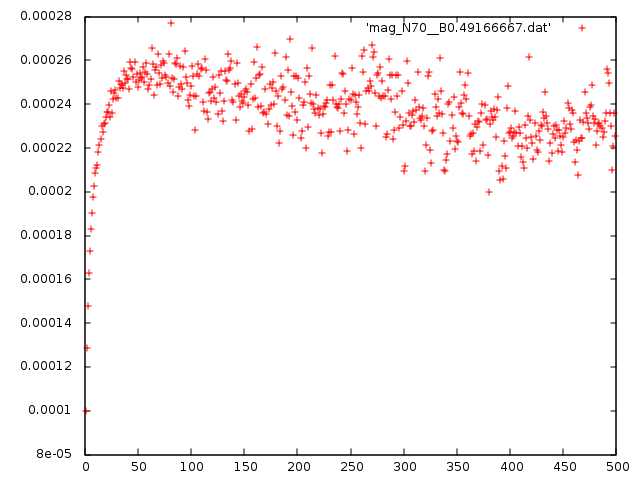
\includegraphics[scale=0.45]{metropolis/bin_mag_049.png}
}
\caption{Deviazione standard della magnetizzazione in funzione della larghezza dei \emph{bin} }
\end{figure}

\newpage
\subsubsection*{Swendsen-Wang}
Si vedano anche per questo algoritmo le stesse osservabili alle stesse temperature di Metropolis. 
\begin{figure}[h!]
\subfigure[Energia a $\beta=0.325$]{
	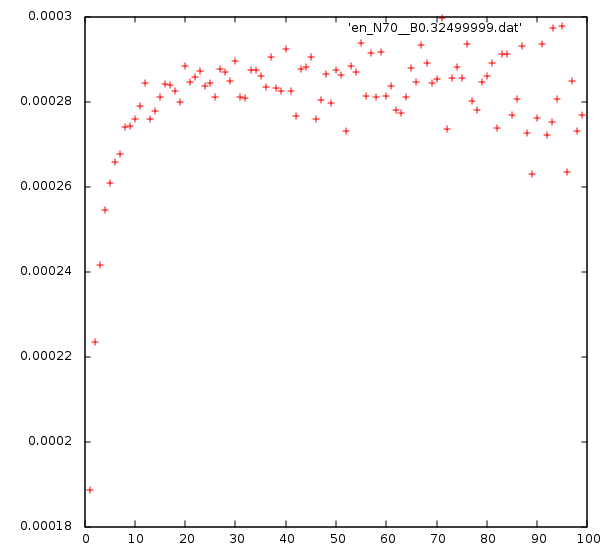
\includegraphics[scale=0.45]{sw/bin_en_0325.png}
}
\subfigure[Energia $\beta=0.4508$]{
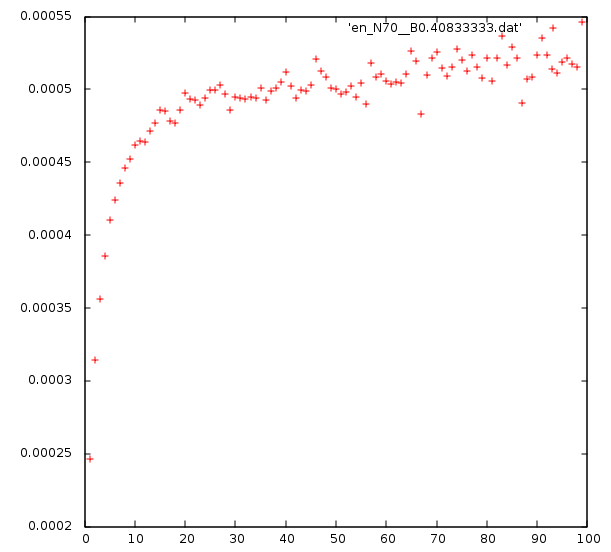
\includegraphics[scale=0.45]{sw/bin_en_0408.png}
}
\caption{Deviazione standard dell'energia in funzione della larghezza dei \emph{bin} }
\end{figure}
\begin{figure}[h!]
\subfigure[Energia a $\beta=0.453$]{
	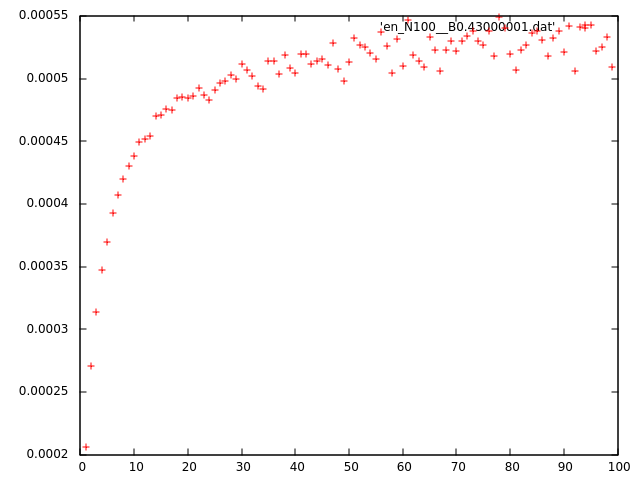
\includegraphics[scale=0.45]{sw/bin_en_043.png}
}
\subfigure[Energia $\beta=0.459$]{
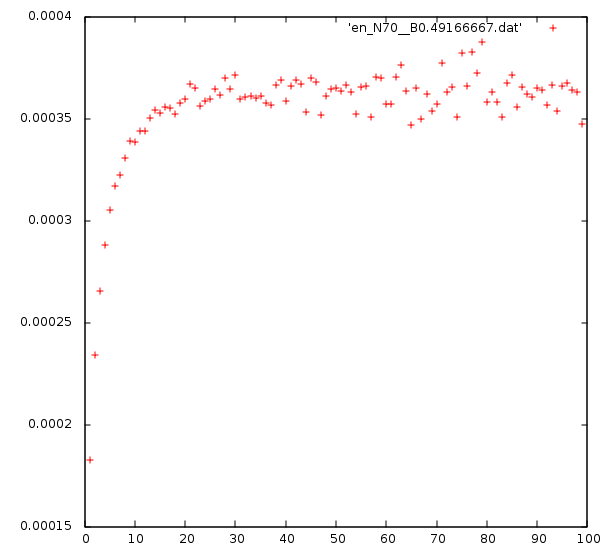
\includegraphics[scale=0.45]{sw/bin_en_049.png}
}
\caption{Deviazione standard dell'energia  in funzione della larghezza dei \emph{bin} }
\end{figure}


\begin{figure}[h!]
\subfigure[Magnetizzazione a $\beta=0.325$]{
	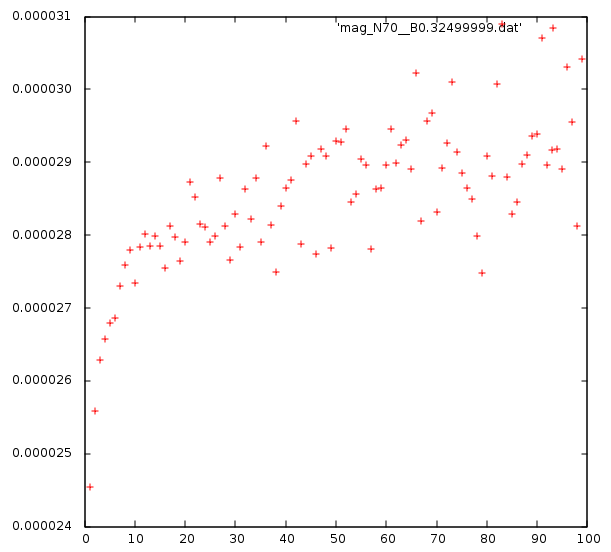
\includegraphics[scale=0.45]{sw/bin_mag_0325.png}
}
\subfigure[Magnetizzazione $\beta=0.4508$]{
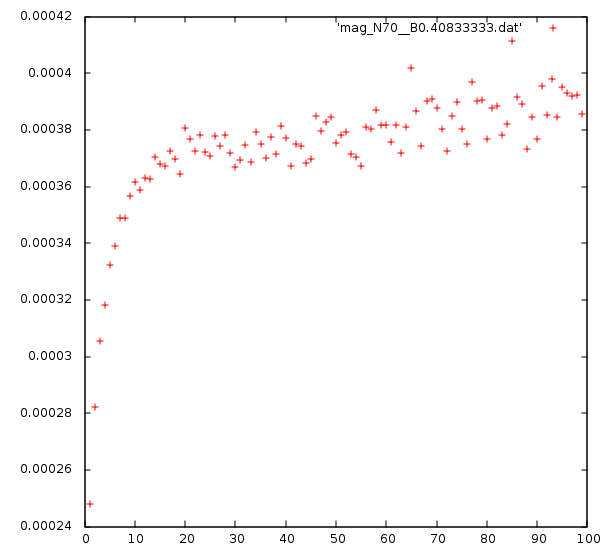
\includegraphics[scale=0.45]{sw/bin_mag_0408.png}
}
\caption{Deviazione standard della magnetizzazione in funzione della larghezza dei \emph{bin} }
\end{figure}
\begin{figure}[h!]
\subfigure[Magnetizzazione a $\beta=0.43$]{
	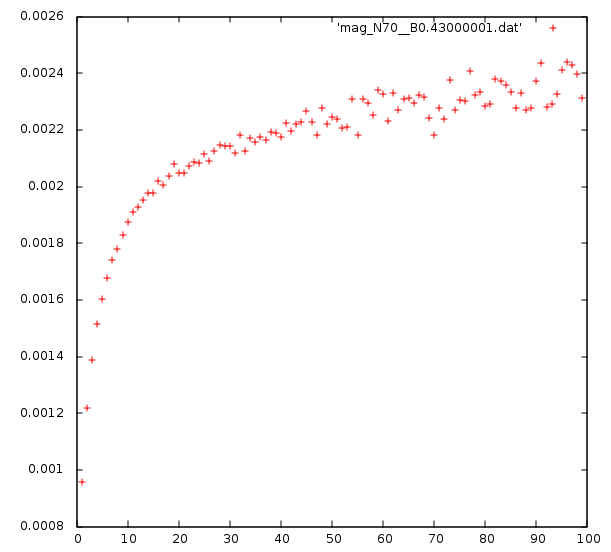
\includegraphics[scale=0.45]{sw/bin_mag_043.png}
}
\subfigure[Magnetizzazione $\beta=0.49$]{
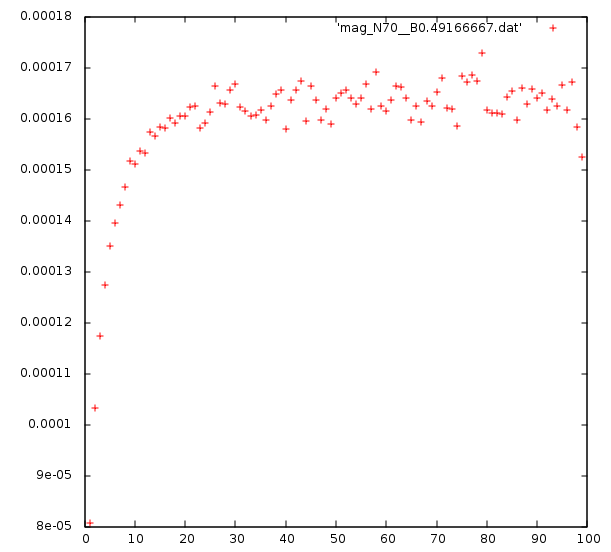
\includegraphics[scale=0.45]{sw/bin_mag_049.png}
}
\caption{Deviazione standard della magnetizzazione in funzione della larghezza dei \emph{bin} }
\end{figure}

Come si può vedere da un confronto diretto dei grafici, analizzando il valore per cui la curva di appiattisce, si può notare che, come ci si poteva aspettare, nell'algoritmo Metropolis è necessario scegliere una larghezza dell'intervallo molto alta vicino al punto critico, addirittura un ordine di grandezza superiore rispetto a Swendsen-Wang.
Si stima la larghezza ottimale dell'intervallo cercando il punto in cui la curva si appiattisce o inizia ad avere una derivata prima molto più piccola rispetto ai punti iniziali.
Si può vedere inoltre, come avvicinandosi al punto critico sia necessario avere un intervallo più largo: ciò è una chiara conseguenza della crescita di $\tau_{corr}$ all'avvicinarsi al punto critico.\\
Inoltre, prendiamo l'esempio del caso metropolis. Alla temperatura $\beta = 0.325$ possiamo prendere come larghezza del bin 20. Poco sotto il punto critico, avremo come larghezza bin ~ 150/200. Come nel caso dell'autocorrelazione avvicinandosi del punto critico la quantità in questione è aumentata di circa un fattore 10 in entrambi i casi.
Ciò può far capire perchè tempo di autocorrelazione e larghezza del bin siano due quantità non indipendenti.\\
A riprova di ciò, si può fare la stessa analisi con Swendsen-Wang: si passa da un larghezza del bin di circa 10 a una larghezza di circa 20. Esso è aumentato di un fattore simile al tempo di autocorrelazione, che è passato da 2.5 a 5.5 .\\
In seguito a questa analisi è stata scelta come larghezza dei bin per Metropolis  200 e per Swendsen-Wang 30.\\
Per via di questa grande differenza di larghezza dei bin il numero di passi temporali eseguiti con Metropolis è stato aumentato a 120000, mentre Swendsen-Wang rimane con 20000 passi in modo da avere errori più simili con i due algoritmi. In questo modo infatti si ha un numero di misure molto simile dopo il binning.\\
Nonostante Metropolis sia molto più veloce di Swendsen-Wang a parità di step temporali, la grande autocorrelazione fra le configurazioni generate impone di dover generare molte più configurazioni. Questo fatto lo rende più lento di Swendsen-Wang a generare un sample di dati simili.\\
Si confrontino i tempi dei due algoritmi in un reticolo 100x100:
\\
\begin{center}
\begin{tabular}{cc}
\toprule
	Metropolis (120000 step) & Swendsen-Wang (20000 step) \\
\midrule
	111 s & 48 s \\
\bottomrule
\end{tabular} 
\end{center}

L'algoritmo Swendsen-Wang risulta così più efficiente di Metropolis.
\newpage

\subsection{Energia e Magnetizzazione}
Energia e magnetizzazione sono le due principali osservabili di questo modello ed è possibile confrontare facilmente il loro andamento con la soluzione teorica di Onsager (valida però per un reticolo di taglia infinita).
Per la magnetizzazione è stata utilizzata l'osservabile \emph{improved} per Swendsen-Wang, ossia la frazione degli spin nel cluster più grande.
Nonostante i grafici siano stati fatti con un reticolo 100x100 l'accordo con la previsione teorica è eccellente per entrambe le osservabili e con entrambi gli algoritmi.
Insieme ai dati raccolti è stata sovrapposta la soluzione analitica di Onsager per entrambe le osservabili.
\begin{figure}[h]
	\subfigure[Metropolis]{
		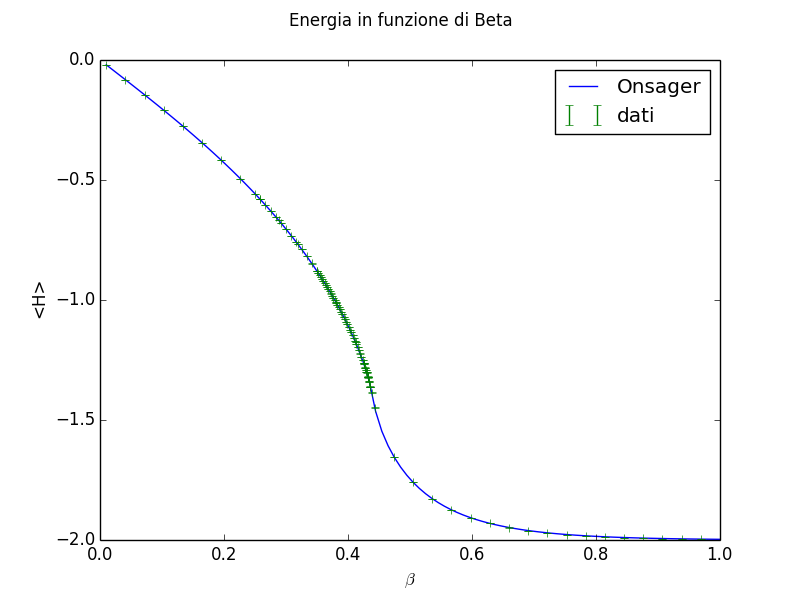
\includegraphics[scale=0.35]{metropolis/en_beta.png}
	}
	\subfigure[Swendsen-Wang]{
		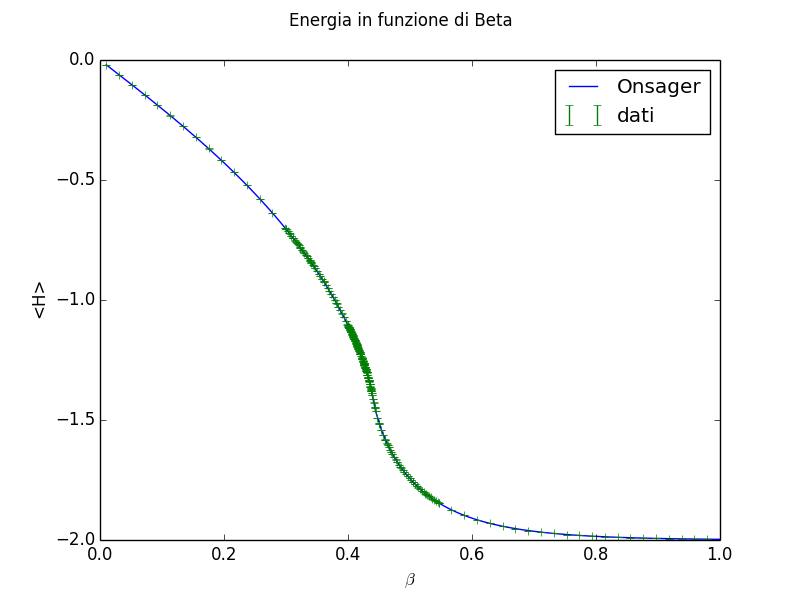
\includegraphics[scale=0.35]{sw/en_beta.png}
	}
\caption{Energia in funzione di $\beta$, 100x100.}
\end{figure}

\begin{figure}[h]
	\subfigure[Metropolis]{
		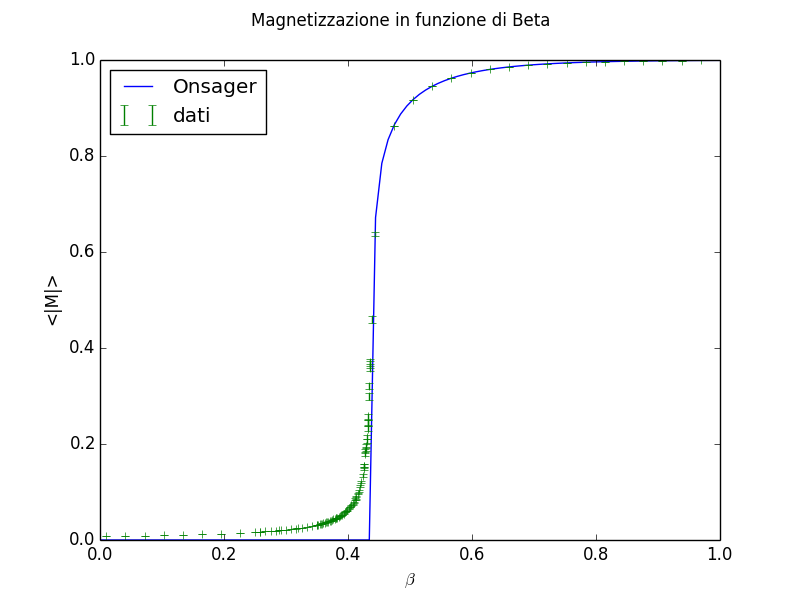
\includegraphics[scale=0.35]{metropolis/mag100.png}
	}
	\subfigure[Swendsen-Wang]{
		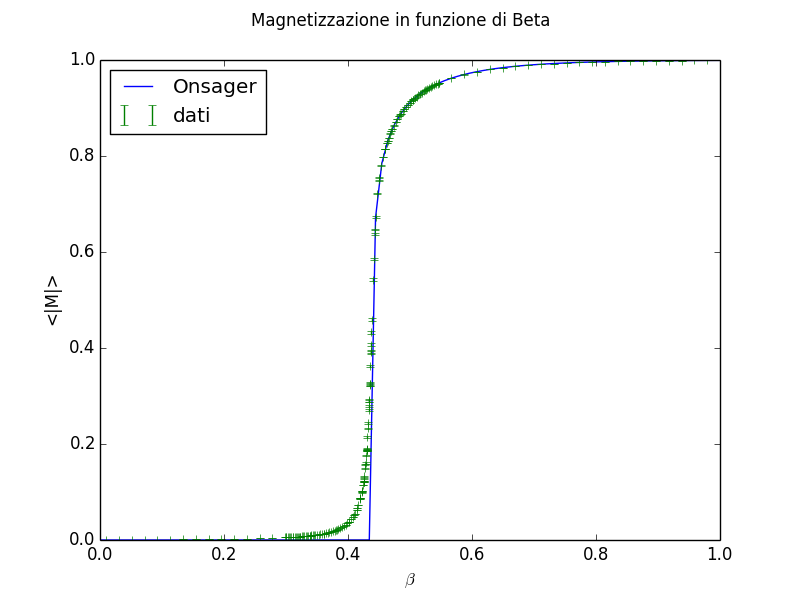
\includegraphics[scale=0.35]{sw/mag100.png}
	}
\caption{Magnetizzazione in funzione di $\beta$, 100x100.}

\end{figure}

Gli errori sono stati calcolati attraverso il binning delle osservabili.
\subsection{Distribuzione di probabilità della magnetizzazione}
Si studi ora la distribuzione di probabilità del modulo della magnetizzazione al variare della temperatura, confrontando fra loro i due algoritmi in questione.
Si è deciso di studiare il modulo della magnetizzazione in quanto l'algoritmo Swendsen-Wang ad ogni step inverte i cluster (con probabilità $\frac{1}{2}$), mentre Metropolis, siccome inverte uno spin alla volta, tende a mantere costante il segno della magnetizzazione per temperature sotto il punto critico.


\begin{figure}
	\subfigure[ $\beta=0.3$]{
		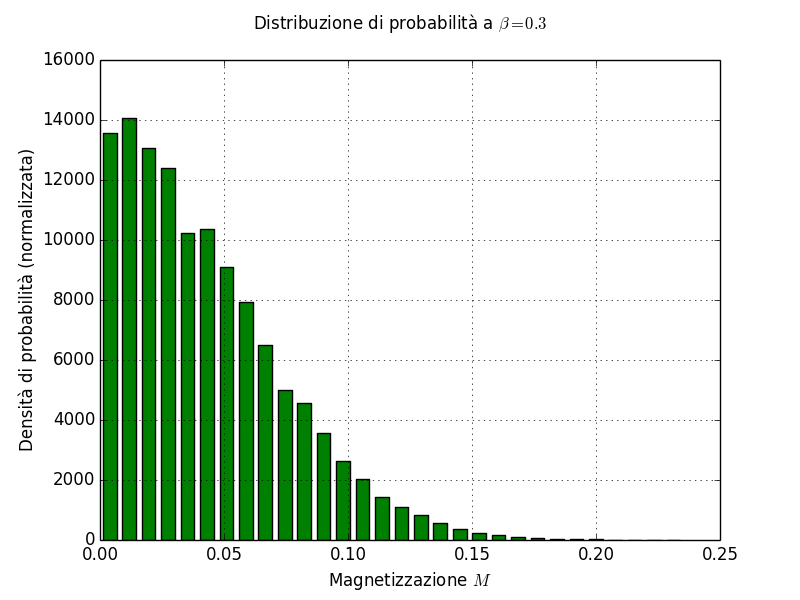
\includegraphics[scale=0.36]{metropolis/PDFM03.png}	
	}
	\subfigure[ $\beta=0.42$]{
		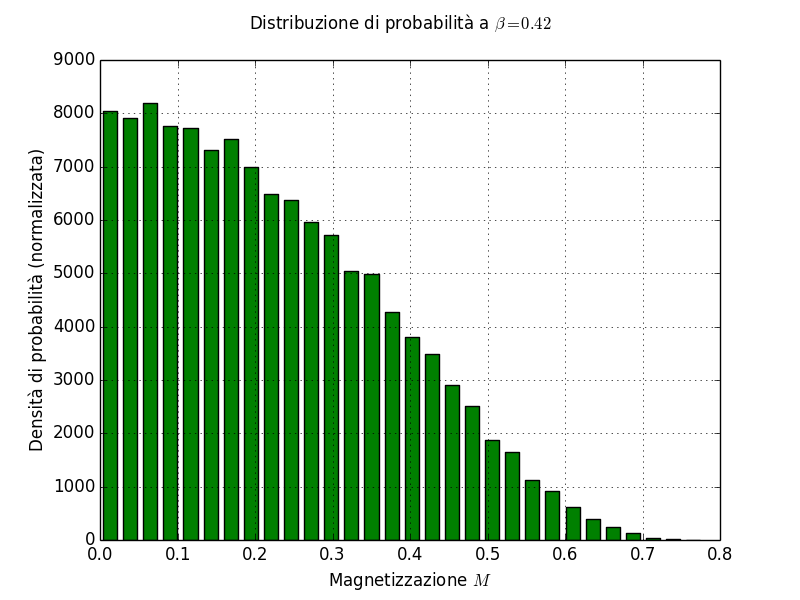
\includegraphics[scale=0.36]{metropolis/PDFM042.png}	
	}
	\caption{Metropolis}
\end{figure}
\begin{figure}
	\subfigure[ $\beta=0.43$]{
		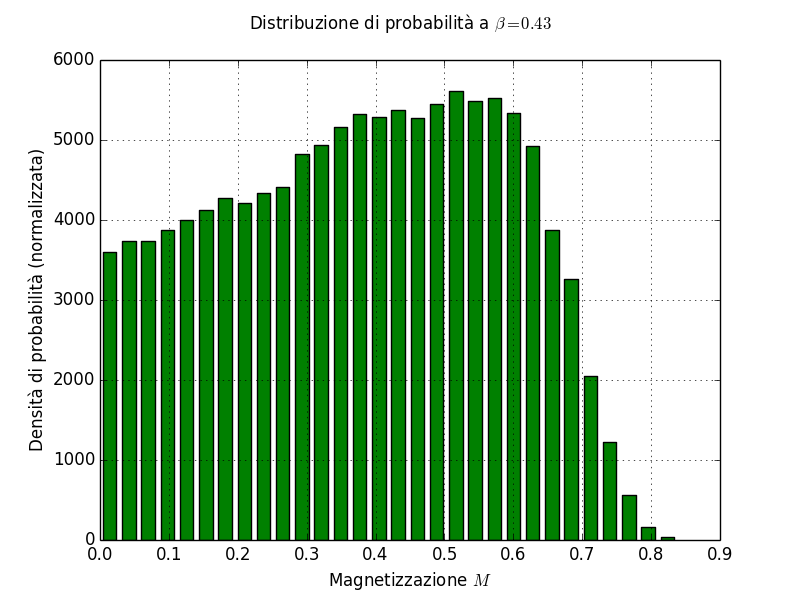
\includegraphics[scale=0.36]{metropolis/PDFM043.png}	
	}
	\subfigure[ $\beta=0.44$]{
		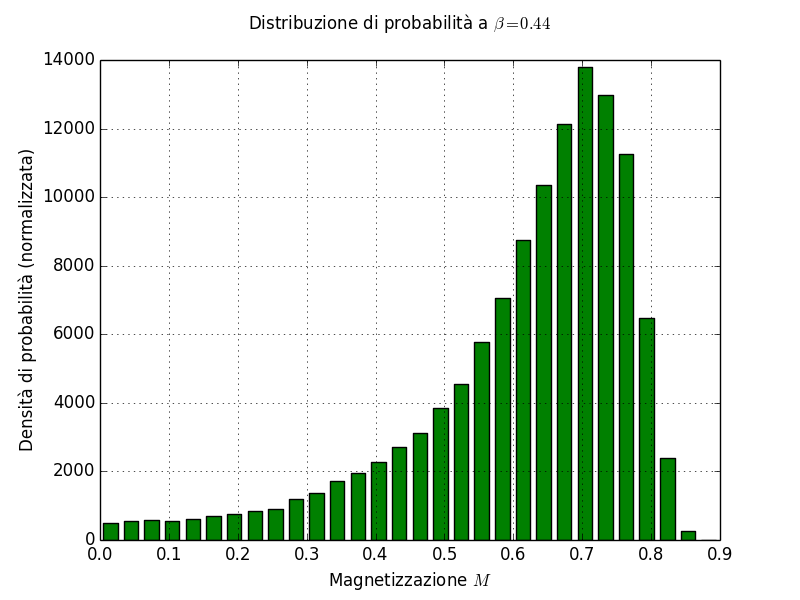
\includegraphics[scale=0.36]{metropolis/PDFM044.png}	
	}
	\caption{Metropolis}
\end{figure}

\begin{figure}
	\subfigure[ $\beta=0.46$]{
		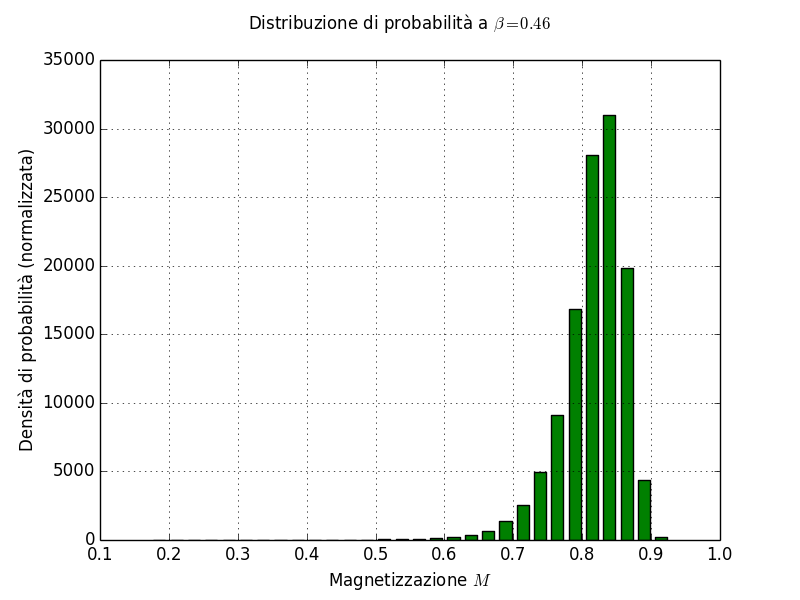
\includegraphics[scale=0.36]{metropolis/PDFM046.png}	
	}
	\subfigure[ $\beta=1$]{
		\includegraphics[scale=0.36]{metropolis/PDFM1.png}	
	}
	\caption{Metropolis}
\end{figure}


\begin{figure}
	\subfigure[ $\beta=0.3$]{
		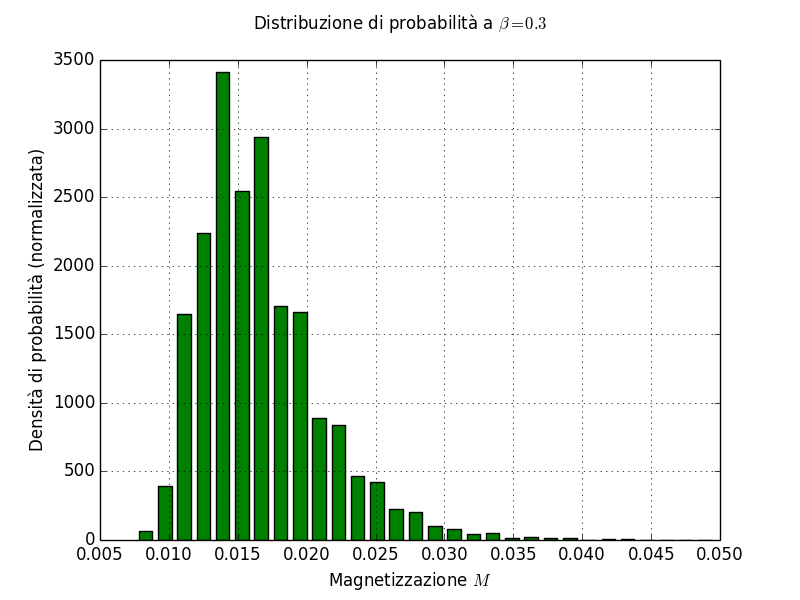
\includegraphics[scale=0.36]{sw/pdfM03.png}	
	}
	\subfigure[ $\beta=0.42$]{
		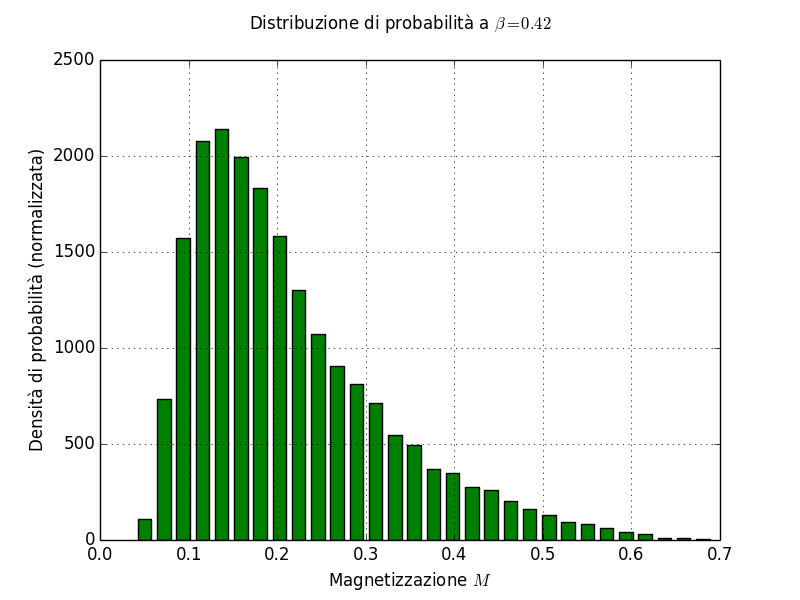
\includegraphics[scale=0.36]{sw/pdfM042.png}	
	}
	\caption{Swendsen-Wang}
\end{figure}
\begin{figure}
	\subfigure[ $\beta=0.43$]{
		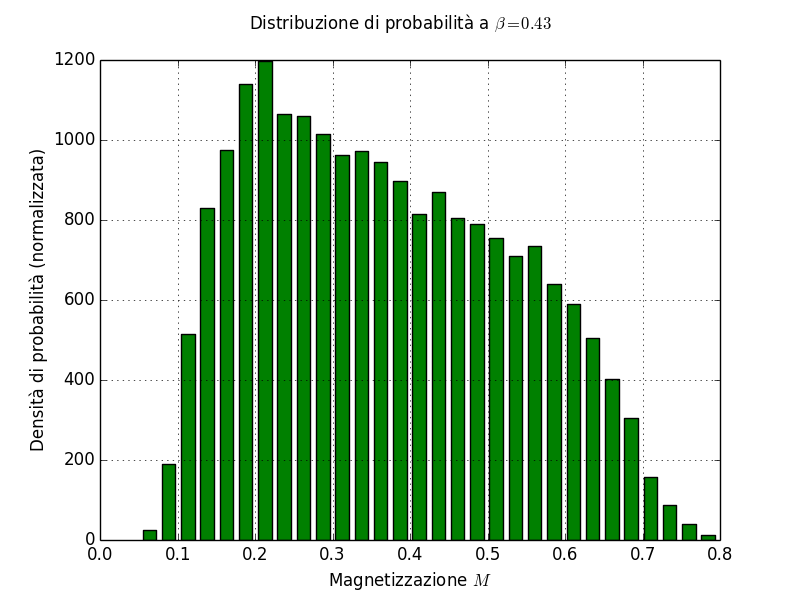
\includegraphics[scale=0.36]{sw/pdfM043.png}	
	}
	\subfigure[ $\beta=0.44$]{
		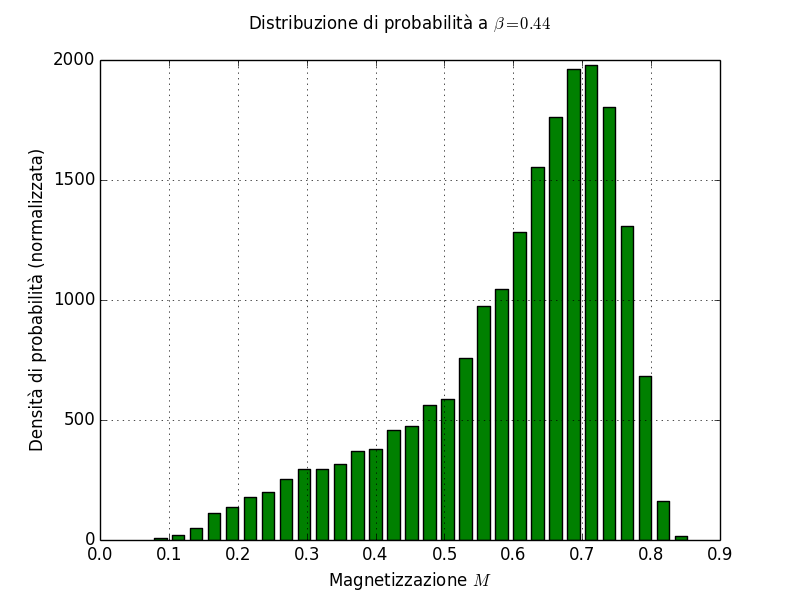
\includegraphics[scale=0.36]{sw/pdfM044.png}	
	}
	\caption{Swendsen-Wang}
\end{figure}

\begin{figure}
	\subfigure[ $\beta=0.46$]{
		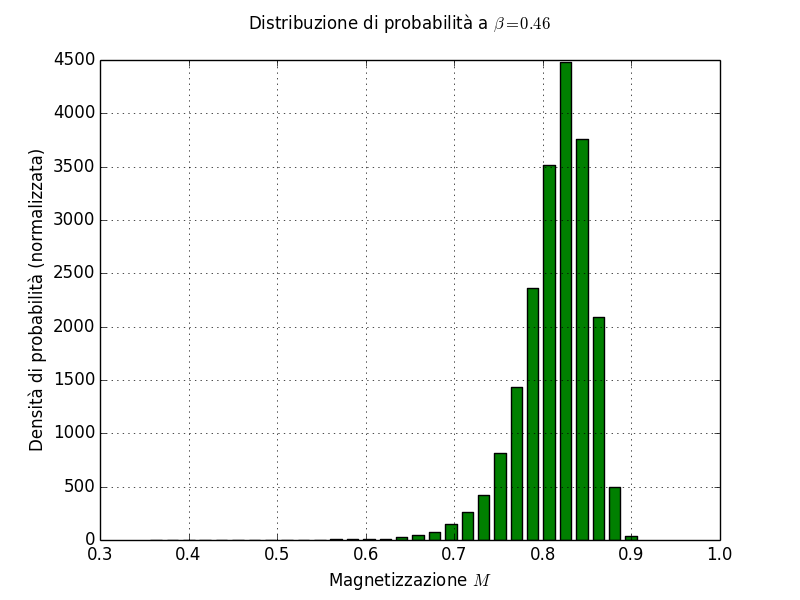
\includegraphics[scale=0.36]{sw/pdfM046.png}	
	}
	\subfigure[ $\beta=1$]{
		\includegraphics[scale=0.36]{sw/pdfM1.png}	
	}
	\caption{Swendsen-Wang}
\end{figure}




\subsection{Lunghezza di correlazione}

La lunghezza di correlazione è stata stimata dal calcolo di:
$$
	<S_0 S_t > \, = \, A \, e^{-\frac{t}{\xi}} \qquad \mbox{dove} \qquad S_n = \frac{1}{L} \sum_i \sigma_{(n,i)} 
$$
Nel calcolo di $<S_0 S_t>$, inoltre è stata sfrutta l'invarianza per traslazione, rotazione di $\frac{\pi}{2}$ e inversione del reticolo, in modo da diminuire l'errore associato a questa grandezza.
Si sfrutta l'invarianza per traslazione calcolando più precisamente la seguente quantità:
$$
	<S_0 S_t> = \frac{1}{L} \sum <S_i S_{t+i}>
$$ 
\begin{figure}[h]
\centering
	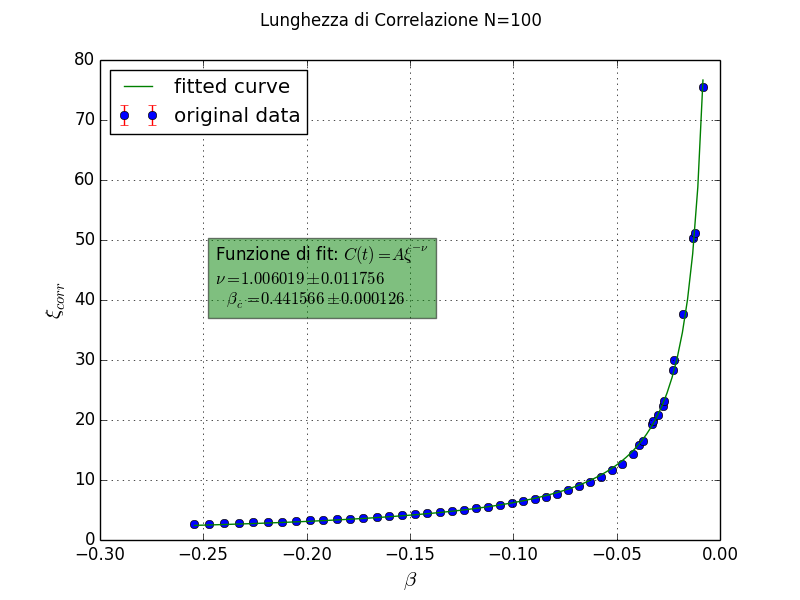
\includegraphics[scale=0.56]{metropolis/corrN100.png}
\caption{Lunghezza di correlazione con algoritmo Metropolis.}
\end{figure}
\begin{figure}[h]
\centering
	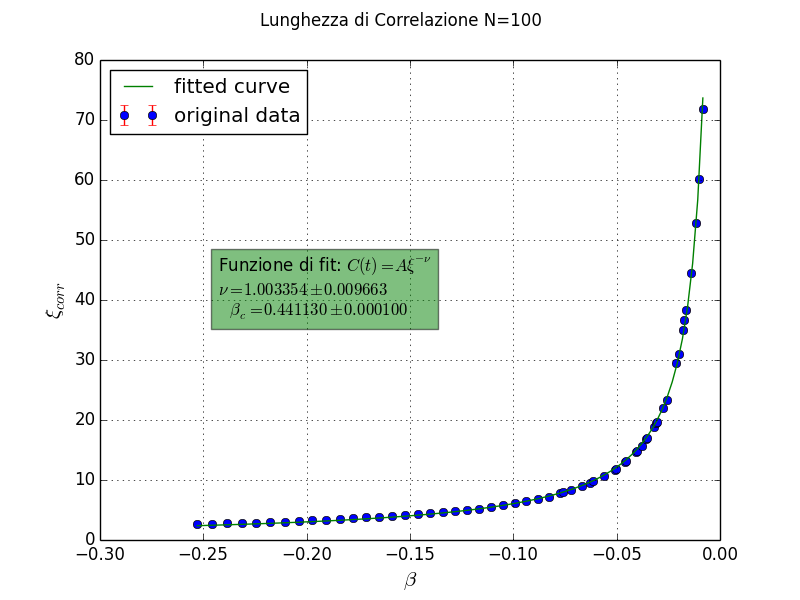
\includegraphics[scale=0.56]{sw/corrN100.png}
\caption{Lunghezza di correlazione con algoritmo Swendsen-Wang.}
\end{figure}
L'invarianza per rotazioni di $\frac{\pi}{2}$ è stata utilizzata mediando il calcolo fra righe e colonne. Inoltre è stata utilizzata anche l'invarianza per inversione  e la ciclicità del reticolo, le quali insieme comportano la validità di questa relazione:
$$
	< S_0 S_t> = < S_0 S_{L-t}>
$$
A questo punto si è calcolata osservabile e si sono stimati gli errori attraverso un binning come per le altre osservabili.
I Valori della lunghezza di correlazione sono poi così stati stimati fittando con un esponenziale decrescente. I valori ottenuti dal fit (errori compresi) sono stati utilizzati per i grafici della lunghezza di correlazione in funzione della temperatura.

Il risultato del fit è quindi:
\begin{center}
	\begin{tabular}{cc}
	\toprule
	Algoritmo & $\nu$ \\
	\midrule
	Metropolis & $ 1.01 \pm 0.01 $\\
	Swendsen-Wang	& $ 1.00 \pm 0.01 $\\
	\bottomrule
	\end{tabular}
\end{center}

Come si può vedere in entrambi i casi l'accordo con la previsione teorica che prevede $\nu = 1$ è ottima per un reticolo 100x100. Inoltre, grazie ad aver imposto un numero di intervalli di binning simile tra i due algoritmi permette di avere una precisione molto simile tra i due.

\newpage
\subsection{Finite Size Scaling}
Si andranno ora a fare uno studio di \emph{finite size scaling} per poter valutare l'accordo dei dati ottenuti per magnetizzazione, suscettività e calore specifico con gli esponenti critici esatti della soluzione di Onsager.
Per fare uno studio di \emph{finite size scaling} è necessario raccogliere dati sulle osservabili in esame per varie taglie del reticolo. In questo caso sono state utilizzati i seguenti reticoli:
\begin{itemize}
\item 30x30 
\item 50x50 
\item 75x75 
\item 100x100 
\end{itemize}
A questo punto, per suscettività e calore specifico è stato necessario calcolare per ognuno di essi la temperatura critica.
Nel caso della suscettività essa è stata ottenuta facendo un fit con una parabola del picco, mentre per magnetizzazione e calore specifico è stata utilizzata la temperatura critica della soluzione analitica.
Questa scelta è dovuta all'impossibilità di ricavare la temperatura critica in modo soddisfacente per il calore specifico attraverso il metodo della parabola.
Per la magnetizzazione questo non è stato necessario in quanto presenta alcun picco.\\
Dopo aver ricavato la temperatura critica, si fa una traslazione sulla temperatura portandola nella nuova variabile 
$$
	 t = \frac{\beta - \beta_{crit}}{\beta}
$$ 
Infine si effettua l'ultimo cambio di variabile, indicando con $L$ la taglia del reticolo e considerando la magnetizzazione si avrà:
\begin{align}
	t \longrightarrow L^{\frac{1}{\nu}} t = L t \\
	M \longrightarrow \frac{M}{L^{\frac{-\beta}{\nu}}} = \frac{M}{L^{-\beta}}
\end{align}
Riguardo alla suscettività invece:
$$
	\chi \longrightarrow \frac{\chi}{L^{\frac{\gamma}{\nu}}} = \frac{\chi}{L^{\gamma}}
$$
Nel caso del calore specifico, la soluzione analitica prevede che abbia esponente $\alpha=0$ il che indica uno scaling di tipo logaritmo. Per esso l'equazione precedente viene modificata in:
$$
	c \longrightarrow \frac{c}{\log{L}}
$$
Gli esponenti critici della soluzione analitica sono i seguenti:
\begin{center}
	\begin{tabular}{|c|c|}
		\toprule
		Esponente & valore \\
		\midrule
		$\alpha$ & 0 \\
		$\beta$ & $1/8$\\
		$\gamma$ & $7/4$ \\
		\bottomrule
	\end{tabular}
\end{center}

\begin{center}
	\begin{figure}[h]
		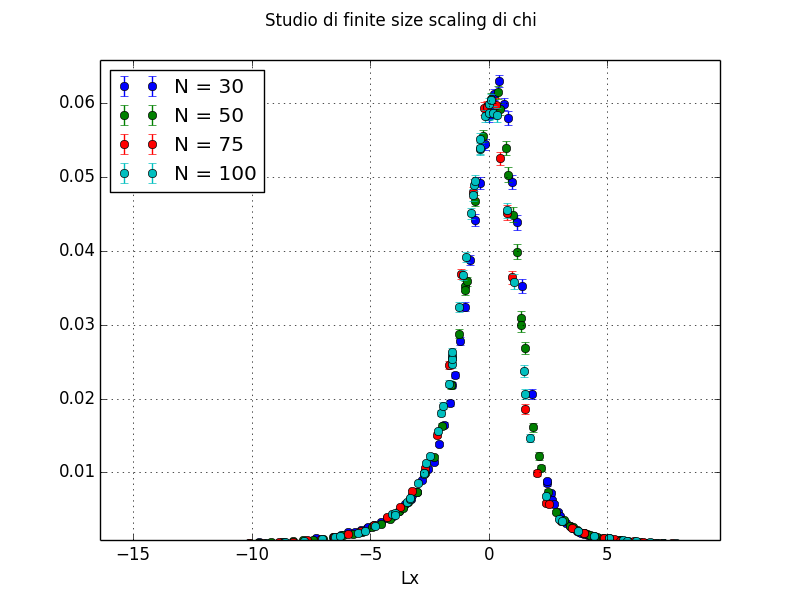
\includegraphics[scale=0.56]{sw/fsschi.png}
		\caption{Studio di Fss per $\chi = t^{-\gamma}$, con $\gamma = \frac{7}{4}$}
	\end{figure}
\end{center}
\begin{center}
	\begin{figure}[h]
		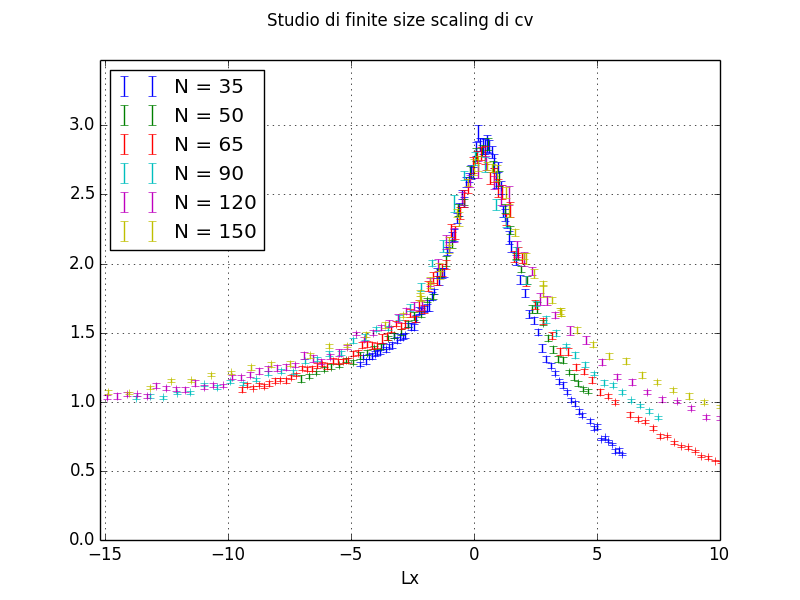
\includegraphics[scale=0.56]{sw/fsscv.png}
		\caption{Studio di Fss per $c$, con $\alpha=0$}
	\end{figure}
\end{center}
\begin{center}
	\begin{figure}[h!]
		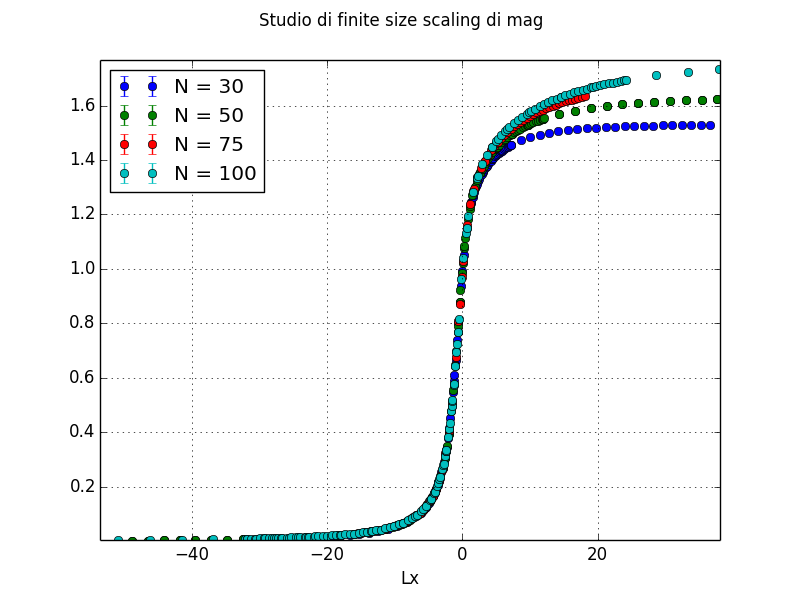
\includegraphics[scale=0.56]{sw/fssmag.png}
		\caption{Studio di Fss per $M= t^{\beta}$, con $\beta=\frac{1}{8}$}
	\end{figure}
\end{center}

A questo punto, ci si aspetta di vedere che le curve per ciascuna taglia, opportunamente scalate nella procedura descritta, collassino su un'unica curva \emph{universale}.
Come si può vedere dai grafici per queste tre osservabili è proprio ciò che accade nella regione paramagnetica con $\beta < \beta_{crit}$.\\
Siccome il \emph{finite size scaling} si basa sugli esponenti critici della soluzione esatta, dal risultato di questa analisi possiamo dire che le osservabili calcolate scalano in modo molto simile a ciò che ci si aspetterebbe teoricamente.
Per questo, gli esponenti critici del modello simulato sembrano risultare simili a quelli previsti teoricamente.

\newpage
\section{Modello di Potts}
Il modello di Potts è una generalizzazione del modello di Ising studiato nel capitolo precedente.
Esso generalizza il modello di Ising aggiungendo un numero arbitrario di stati.

\end{document}
